\section{Finding the Optimal Values for Linear Regression Coefficients}

Let us return to our data frame \texttt{df}. The column \texttt{Input\_Variable(X)} serves as our predictor variable.
The variable \texttt{Actual\_Output(yact)}, as its name indicates, is the true target output variable.

Using these two variables, we can empirically compute the values of $\a$ and $\beta$ according to equations \eqref{alfa} and \eqref{beta}. In the following Python script, we implement these exact formulas to derive an optimal linear regression model.

[,]{\texttt{optimalValue.py}}
\begin{lstlisting}[language=Python]
#!/usr/bin/env python3
# -*- coding: utf-8 -*-
"""
Created on Mon Oct 23 00:37:36 2017

@author: jdk2py
"""

import pandas as pd
import numpy as np

np.random.seed(1234)

x = 2.5 * np.random.randn(100) + 1.5
res = .5 * np.random.randn(100) + 0
ypred = 2 + .3 * x
yact = 2 + .3 * x + res
xlist = x.tolist()
ypredlist = ypred.tolist()
yactlist = yact.tolist()
df = pd.DataFrame({'Input_Variable(X)': xlist, 'Predicted_Output(ypred)': ypredlist, 'Actual_Output(yact)': yactlist})

ymean = np.mean(yact)
yavg = [ymean for i in range(1, len(xlist) + 1)]

import matplotlib.pyplot as plt

xmean = np.mean(df['Input_Variable(X)'])
ymean = np.mean(df['Actual_Output(yact)'])
df['betan'] = (df['Input_Variable(X)'] - xmean) * (df['Actual_Output(yact)'] - ymean)
df['xvar'] = (df['Input_Variable(X)'] - xmean) ** 2
betan = df.sum()['betan']
betad = df.sum()['xvar']
beta = betan / betad
alpha = ymean - beta * xmean
print(beta, alpha)

df['ymodel'] = beta * df['Input_Variable(X)'] + alpha

df['SSR'] = (df['ymodel'] - ymean) ** 2
df['SST'] = (df['Actual_Output(yact)'] - ymean) ** 2
SSR = df.sum()['SSR']
SST = df.sum()['SST']
R2 = SSR / SST

print(df.head())

plt.plot(x, ypred)
plt.plot(x, df['ymodel'], "b")
plt.plot(x, yact, 'ro')
plt.plot(x, yavg)
plt.title('Actual vs Predicted vs Model')
\end{lstlisting}

[,]{Screen Output}
\begin{lstlisting}[language=Python]
   Actual_Output(yact)  Input_Variable(X)  Predicted_Output(ypred)     betan  \
0             2.949179           2.678588                 2.803576  0.543137
1             1.840035          -1.477439                 1.556768  1.873530
2             3.776326           5.081767                 3.524530  4.629773
3             2.358159           0.718370                 2.215511  0.080941
4             2.151703          -0.301472                 1.909558  0.565934

       xvar    ymodel       SSR       SST
0  1.189860  2.796261  0.119028  0.247926
1  9.395573  1.481781  0.939885  0.373592
2 12.207943  3.556345  1.221220  1.755808
3  0.755875  2.176277  0.075614  0.008667
4  3.569275  1.853719  0.357052  0.089733
\end{lstlisting}

\begin{center}
	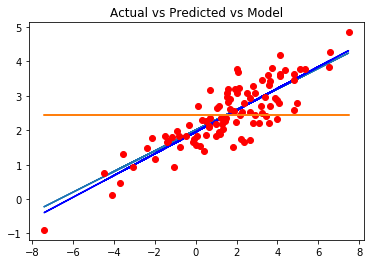
\includegraphics[width=10cm,keepaspectratio=true]{./images/optimalValue.png}
\end{center}

In addition to the $R^2$ metric, there are other critical statistics and parameter diagnostics that one must examine to accomplish the following:

\begin{enumerate}
	\item Select specific candidate variables and discard redundant ones from the model.
	\item Evaluate the empirical relationship between a predictor and the target outcome, rigorous testing whether a given variable is statistically significant within the model.
	\item Quantify the expected prediction error of the finalized model.
\end{enumerate}

Let us now examine some of the statistical tests and diagnostics designed to address the considerations discussed above.

It is crucial to note that when we compute the sample values of $\a$ and $\beta$, we obtain point estimates rather than exact population parameters. Therefore, we must formally demonstrate their statistical significance using a hypothesis test.

This hypothesis test evaluates whether the true population slope parameter $\beta$ is significantly different from zero. In other words, it tests whether a real linear association exists between $X$ and $Y$. If such a relationship exists, then $\beta \neq 0$.

In the linear equation $y = \a + \beta x$, if we set $\beta = 0$, any linear relationship between $x$ and $y$ vanishes. Consequently, our formal hypothesis test is structured as:
\begin{align}
	\texttt{Null Hypothesis } H_0: \beta &= 0 \\
	\texttt{Alternative Hypothesis } H_a: \beta &\neq 0
\end{align}

In statistical practice, when a linear regression is executed and $\beta$ is estimated, this output is accompanied by a $t$-statistic and its corresponding $p$-value.

As we will see shortly, Python statistical packages provide built-in methods to compute this exact $p$-value automatically.

Our task then consists of comparing this computed $p$-value against a pre-selected significance level ($\alpha$).

Because the alternative hypothesis $\beta \neq 0$ can be decomposed into two distinct directions:
\begin{align}
	\beta > 0 \texttt{ or } \beta < 0,
\end{align}
this constitutes a two-tailed test. If the resulting $p$-value is less than our threshold significance level, we reject the null hypothesis $H_0: \beta = 0$ and conclude that $\beta$ is statistically significant.

Conversely, if the $p$-value exceeds our threshold, we fail to reject the null hypothesis, indicating that $\beta$ lacks statistical significance within our model.

As we will see when dealing with multiple linear regression, this behavior guides feature selection by enabling us to drop uninformative columns: the higher the $p$-value, the less significant that variable is to the model, and vice versa.

When transitioning from simple linear regression to multiple linear regression, there will be multiple partial regression coefficients $\beta_1, \beta_2, \dots, \beta_p$, each representing a distinct parameter estimate.

In that general setting, beyond testing the individual statistical significance of each variable (by checking the $p$-values associated with individual $t$-statistics), we must also test whether all slope coefficients simultaneously equal zero as a collective group.

This global test is formulated as follows:
\begin{align}
	\texttt{Null Hypothesis } & H_0: \beta_1 = \beta_2 = \dots = \beta_p = 0 \\
	\texttt{Alternative Hypothesis } & H_a: \exists \beta_i \neq 0
\end{align}

The test statistic utilized for this joint hypothesis test is called the \emph{$F$-statistic}, and it is defined as:
\begin{align}
	F = \dfrac{\left( SST - SSD \right) / p}{SSD / \left( n - p - 1 \right)}
\end{align}

This statistic follows the Snedecor $F$-distribution with $p$ and $n - p - 1$ degrees of freedom.
There is a specific $p$-value associated with this $F$-statistic; if this joint $p$-value is sufficiently small (below the significance level), we reject the null hypothesis and conclude that at least one predictor variable contributes meaningfully to the model.

The critical importance of the $F$-statistic can be summarized as follows:
\begin{itemize}
	\item Individual $t$-test $p$-values reflect marginal relationships between a single predictor and the response. In the presence of multiple predictors, these individual relationships can shift due to inter-variable correlations.
	\item \emph{The $F$-statistic provides a comprehensive assessment of the joint explanatory power gained by the collective set of predictor variables.}
	\item When the total number of candidate predictors ($p$) in the model is very large and all true $\beta_i \approx 0$, individual $p$-values by random chance alone might appear statistically significant.
	\item In such scenarios, \emph{relying solely on individual $p$-values might lead us to incorrectly conclude that a relationship exists when none truly does; inspecting the global $F$-statistic and its joint $p$-value safeguards against this false positive error.}
\end{itemize}

[,]{Residual Standard Error}

Another fundamental diagnostic metric to master is the \emph{Residual Standard Error (RSE)}.

For a simple linear regression model ($p = 1$), it is defined as:
\begin{align}
	RSE = \sqrt{\dfrac{1}{n - 2} SSD}
\end{align}
where $n$ represents the total number of observational data points.

In general, for a multiple regression model with $p$ predictors:
\begin{align}
	RSE = \sqrt{\dfrac{SSD}{n - p - 1}}
\end{align}

The \texttt{RSE} provides an unbiased point estimate of the standard deviation ($\sigma$) of the random error term ($\epsilon$).

This represents the inherent baseline uncertainty that remains unavoidable even if the true population regression coefficients are perfectly known.

Such residual error arises because the model inherently simplifies reality, omitting latent variables or unmeasured structural dynamics.

While we have focused primarily on a single explanatory variable up to this point, real-world data science challenges almost always involve multiple regression, where multiple input variables simultaneously predict the output response.

In multiple regression, the \texttt{RSE} generally decreases as we incorporate informative predictors that explain substantial portions of the target variance.

The exact \texttt{RSE} value for any model can be computed directly using the following Python code snippet, where we calculate \texttt{RSE} for our simulated data frame \texttt{df}:

\begin{lstlisting}[language=Python]
n = len(df['Input_Variable(X)'])
df['SSD'] = (df['Actual_Output(yact)'] - df['ymodel']) ** 2
SSD = df.sum()['SSD']
RSE = np.sqrt(SSD / (n - 2))
\end{lstlisting}

The resulting \texttt{RSE} value in this specific simulation is $\approx 0.4925$. As intuitive common sense dictates, \emph{the smaller the \texttt{RSE}, the more accurate the model}. To benchmark this error, we compare it against the mean of the actual data \texttt{yact} ($\approx 2.4512$). An error of $0.4925$ relative to $2.4512$ corresponds to an average prediction discrepancy of $\approx 20.09\%$.
